\documentclass{beamer}
\usetheme{default}

\usepackage{caption}
\usepackage{subcaption}

\title{1 million structure method for photoelectron spectra:\ restricted normal mode sampling, and Dyson orbital transitions}
\author{T.\ Northey}
\begin{document}
\begin{frame}[plain]
    \maketitle
\end{frame}
\begin{frame}{NMM previous work}
	\begin{figure}[H]
	\centering
		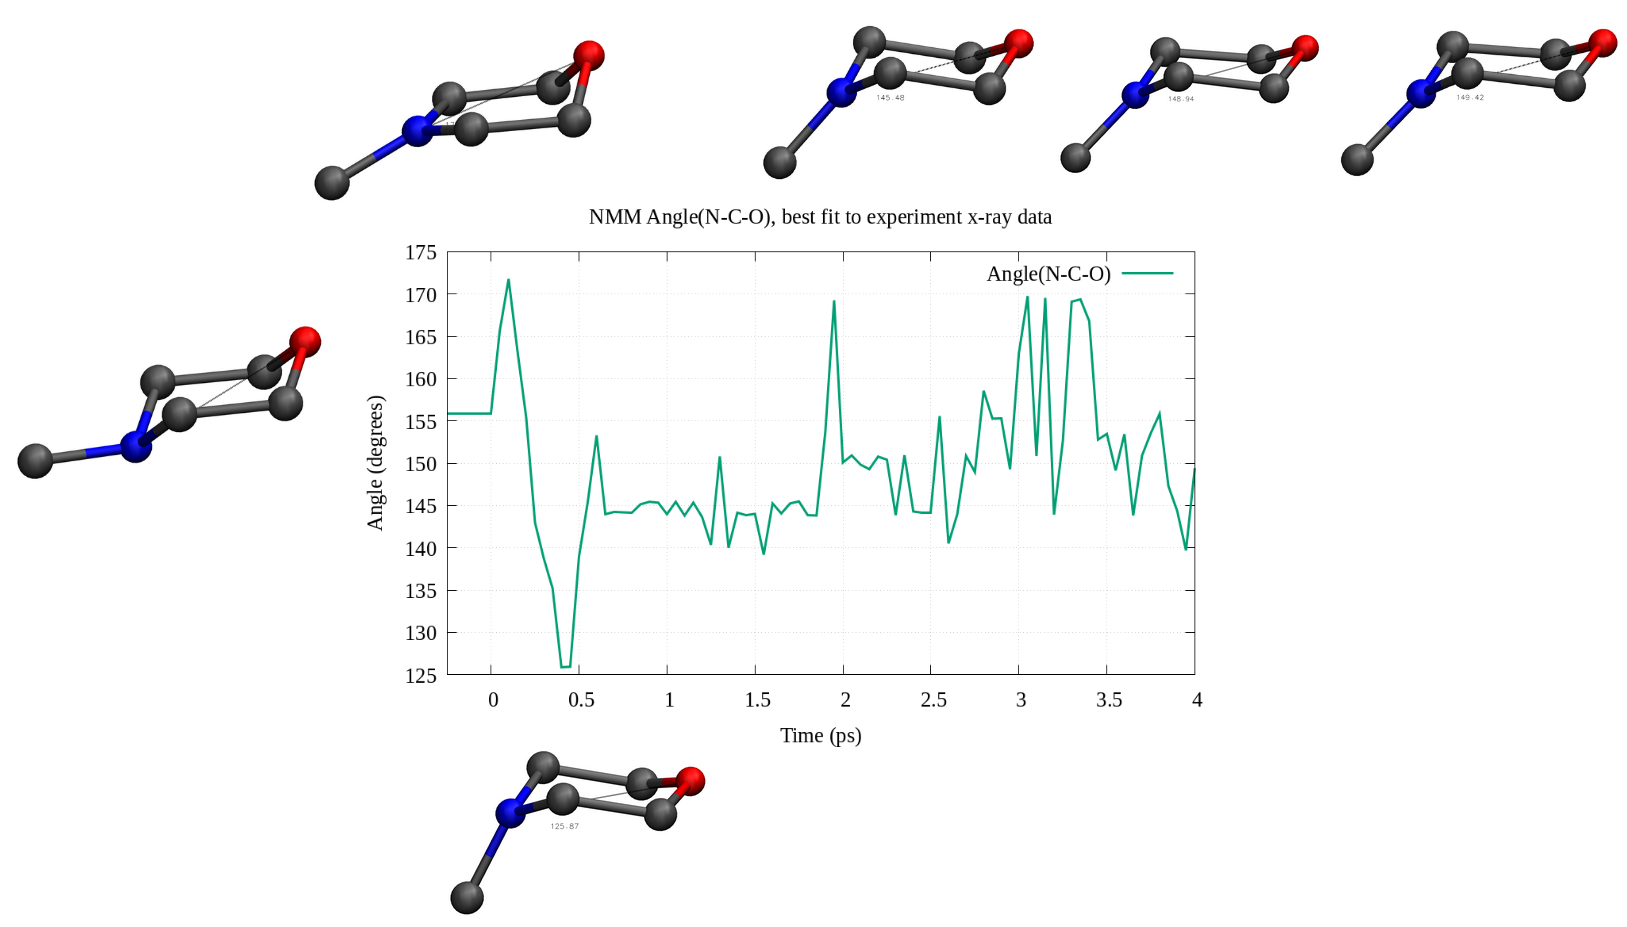
\includegraphics[width=\textwidth]{geomovie_ppt_slide.png}
		\caption{N-C-O angle of best fit to experiment trajectory.}
		\label{fig:geomovie-ppt-slide}
	\end{figure}
	
\end{frame}

\begin{frame}
	\begin{enumerate}
		\item Chlorobenzene has 30 normal modes
		\item Sampling over a selection of 16 `heavy atom' modes effectively clamps the C$-$H bonds (fig.\ \ref{fig:ch_hist}) while keeping the other distances similar (above figures)
		\item Doing this slightly restrains the C$-$C bonds (fig.\ \ref{fig:c1c2_hist}), but only by a difference in fwhm $\simeq$ 0.02 \AA.
		\item I used a sample size of 10,000 molecular structures for the above figures.
	\end{enumerate}
\end{frame}

\begin{frame}{Chlorobenzene normal mode sampling, vary sample size $N$}

\begin{itemize}
	\item From bond-distances statistics, it seems that $N=1000$ and $N=10000$ agree relatively closely. $N=10000$ gives a smoother bell curve distribution for inter-atomic distances.
	\item These samples were generated using all normal modes.
\end{itemize}
\end{frame}

\begin{frame}{Sampling method}
The sampling equation for generating the displaced molecular coordinates is,

\begin{eqnarray}
\textbf{R} = \textbf{R}_0 + \sum_i^{\textrm{modes}} a_i\textbf{d}_i
\end{eqnarray}

with starting geometry $\textbf{R}_0$, and displacement unit vectors $\textbf{d}_i$ for each normal mode are obtained from a frequency calculation.  The factors $a_i$ are randomly generated within a bell curve centered at $\mu=0$, and chosen standard deviation, $\sigma$. 
\end{frame}

\begin{frame}{Chlorobenzene Dyson transitions}

\end{frame}

\end{document}
